\documentclass[pdflatex,sn-mathphys-num,iicol]{sn-jnl}

\usepackage{bookmark}
\usepackage{tabularx}
\usepackage{tikz}
\usetikzlibrary{shapes.geometric, shapes.misc, arrows.meta, positioning, calc}
\usepackage{graphicx}
\usepackage{multirow}
\usepackage{amsmath,amssymb,amsfonts}
\usepackage{amsthm}
\usepackage{mathrsfs}
\usepackage[title]{appendix}
\usepackage{xcolor}
\usepackage{textcomp}
\usepackage{manyfoot}
\usepackage{booktabs}

\theoremstyle{thmstyleone}
\newtheorem{theorem}{Theorem}
\newtheorem{proposition}[theorem]{Proposition}
\theoremstyle{thmstyletwo}
\newtheorem{example}{Example}
\newtheorem{remark}{Remark}
\theoremstyle{thmstylethree}
\newtheorem{definition}{Definition}

\raggedbottom

\begin{document}

\title[CNN Piano Chord Recognition Under Factorized Domain Shift]{Evaluating a CNN for Piano Chord Recognition Under Factorized Acoustic Domain Shift}

\author*[1]{\fnm{Cikal} \sur{Gemintang Seya}}\email{cikalgemintangseya1@gmail.com}

\author[1]{\fnm{Jasman} \sur{Pardede}}\email{jasman@itenas.ac.id}

\affil*[1]{\orgdiv{Informatics}, \orgname{National Institute of Technology}, \orgaddress{\street{Neglasari}, \city{Bandung}, \postcode{40124}, \state{West Java}, \country{Indonesia}}}

\abstract{Isolated piano-chord audio is a 36-class recognition problem: 12 roots $\times$ three interval templates (major, minor, diminished). How a fixed classifier behaves when only one recording factor changes is still poorly measured. We study Constant-Q Transform (CQT) features with a compact Convolutional Neural Network (CNN). The model is trained on a Techno T-9890i keyboard recorded with a tablet microphone and never updated. Evaluation isolates device shift (same Techno, ThinkPad, Vivo, and Flow X13 mics) from instrument shift (Yamaha PSR-S910 on the ThinkPad and Flow mics), then applies eval-only overlays of ESC-50 interior noise, indoor room impulse responses (RIR), and six microphone device impulse responses (DIR). In-domain 5-fold cross-validation is 1.00. Device-only accuracy stays high (0.944--0.994). Switching to the Yamaha is the main recorded drop (0.874--0.885). Synthetic noise cuts accuracy by 0.8--4.9 percentage points. RIR and DIR effects are smaller and sometimes raise accuracy. Residual errors stay on classes that share two notes or differ by one semitone, above all $E$ dim.}

\keywords{Constant-Q Transform, Convolutional Neural Network, generalization, domain shift}

\maketitle

\section{Introduction}\label{sec1}

Recognizing musical chords directly from raw audio is a foundational task in music information retrieval (MIR), underpinning applications such as automatic music transcription, interactive music education tools, and real-time performance feedback systems \cite{Telila2023}\cite{Saputra2021}\cite{Moysis2023}. Unlike symbolic or MIDI-based chord recognition, audio-based recognition must contend with the acoustic realities of sound production: a chord played on one instrument, in one room, captured by one microphone, does not produce the same waveform as the identical chord played on a different instrument, in a different room, captured by a different microphone. This variability is the central obstacle to deploying chord recognition systems in real-world settings, where the recording conditions encountered at inference time are rarely identical to those under which a model was trained \cite{Kusaka2024}.

This mismatch is termed acoustic domain shift and is primarily driven by three factors. First, instrument variation, where differing voice synthesis alter timbre and displace chord vectors in the feature space \cite{Kusaka2024}\cite{Majchrzak2025}. Second, environmental noise, which introduces room acoustics and ambient spectral energy that are absent during training \cite{Majchrzak2025}. Lastly, recording device variation, where microphone frequency responses introduce hardware-induced spectral distortions \cite{Kusaka2024}. Classification errors under domain shift are not a symptom of insufficient training data volume: the three factors change the acoustic feature distribution of the test data away from the distribution the classifier was optimized on \cite{Kusaka2024}\cite{Majchrzak2025}.

A joint three-factor shift matches deployment, but one number hides the cause. A phone microphone on the Techno T-9890i and the Yamaha PSR-S910 on a laptop microphone already used for a device test are different problems. Isolating them with independently recorded datasets, then matching them with controlled overlays of additive noise, room impulse responses (RIR), and device impulse responses (DIR), is needed before proposing a remedy.

To study this problem, a feature representation must first be established for the in-domain case. Time-frequency representations that convert audio into image-like matrices, subsequently classified with convolutional architectures, are now the dominant paradigm across audio recognition tasks including environmental sound classification \cite{Wolf-Monheim2025}, acoustic scene classification, speech recognition \cite{Zaman2023}, and music analysis \cite{Moysis2023}. Among these representations, the Constant-Q Transform (CQT) occupies a distinctive position for keyboard and chord audio. Unlike the Short-Time Fourier Transform (STFT), which uses linearly spaced frequency bins, the CQT uses logarithmically spaced bins with a constant quality factor, aligning each bin with a musical semitone \cite{Lacoste2007}. Harmonic interval patterns therefore appear as consistent shapes in the CQT spectrogram, whereas the same intervals appear at different bin spacings under STFT \cite{Li2021}.

Li \cite{Li2021} reported 84.2\% accuracy for CQT-based chord recognition versus 75.3\% for STFT and 80.8\% for CENS chromagrams under identical CNN architectures. Telila et al.\ \cite{Telila2023} further confirmed that CQT-derived features capture piano note frequency structure with 88.2\% frame-level transcription accuracy, and O'Hanlon and Sandler \cite{OHanlon2021} exploited this same musical-scale alignment to design FifthNet. We keep CQT as the input.

The piano chord problem provides a controlled vocabulary for generalization analysis. With 36 classes formed by 12 chromatic root notes and 3 chord qualities (major, minor, diminished), the task requires fine-grained spectral discrimination: major and minor triads differ by a single semitone shift in the third, and diminished triads differ by a further semitone shift in the fifth, corresponding to shifts of one or two CQT frequency bins at the chosen resolution \cite{Harte2010}. A CNN learns spatially localized hierarchical feature detectors whose convolutional kernels respond to small time-frequency neighborhoods \cite{OShea2015}\cite{Purwono2022}, so local interval geometry can survive a global envelope shift from a new microphone or a new piano voice.

Edwards et al.\ \cite{Edwards2024} run the closest controlled piano OOD study, on note-level transcription rather than chords. They re-record MAESTRO on a Yamaha Disklavier, evaluate on MAPS, and degrade test audio with noise, EQ, pitch shift, and reverb. A studio-only model overfits that room; train-time mixing recovers 88.4 MAPS note-onset F1 with no MAPS training audio. Kusaka and Maezawa \cite{Kusaka2024} use a related recipe for mobile AMT. Both papers treat augmentation as a training intervention. We keep the opposite protocol: one clean-trained CQT--CNN, then recorded and synthetic shifts only at evaluation, so each factor's cost is visible before anyone mixes the training set.

Chord papers still grow the vocabulary \cite{Majchrzak2025} or swap in conformers \cite{Akram2025} and attention \cite{Kusaka2024}, test in-domain, and treat OOD as missing data to be patched with synthetic audio \cite{Byambatsogt2020}\cite{Ostermann2023}. What is missing on isolated piano chords is a factorized reading of a fixed CQT--CNN: device change versus keyboard change, then matched eval-only overlays, with no train-time mixing. Contributions:

\begin{enumerate}[1.]
\item A Techno T-9890i training set and five held-out datasets: three device-shift datasets on the same Techno and two Yamaha PSR-S910 keyboard-shift datasets on mics already used for device tests.
\item Shared CQT features ($216 \times 188 \times 1$), used unchanged by the CNN and by every degradation experiment.
\item Fixed-model CNN evaluation that isolates device change from keyboard change, then ESC-50 interior noise, indoor RIRs, and microphone DIRs applied only at evaluation time.
\end{enumerate}

\section{Methodology}\label{sec3}

Fig.~\ref{fig:methodology} shows the pipeline: dataset acquisition, CQT extraction, CNN training, in-domain cross-validation, recorded out-of-domain evaluation, and eval-only synthetic degradation. Software: Python 3.10, TensorFlow 2.15, scikit-learn 1.7.2, Librosa 0.11.0, NumPy 1.26.4, Matplotlib 3.10.8. Hardware: ASUS ROG Flow X13 (Ryzen 7 6800HS, RTX 3050 Ti, 16\,GB RAM) and Google Colaboratory (T4/A100).

\begin{figure}[t]
  \centering
  \resizebox{0.90\columnwidth}{!}{%
  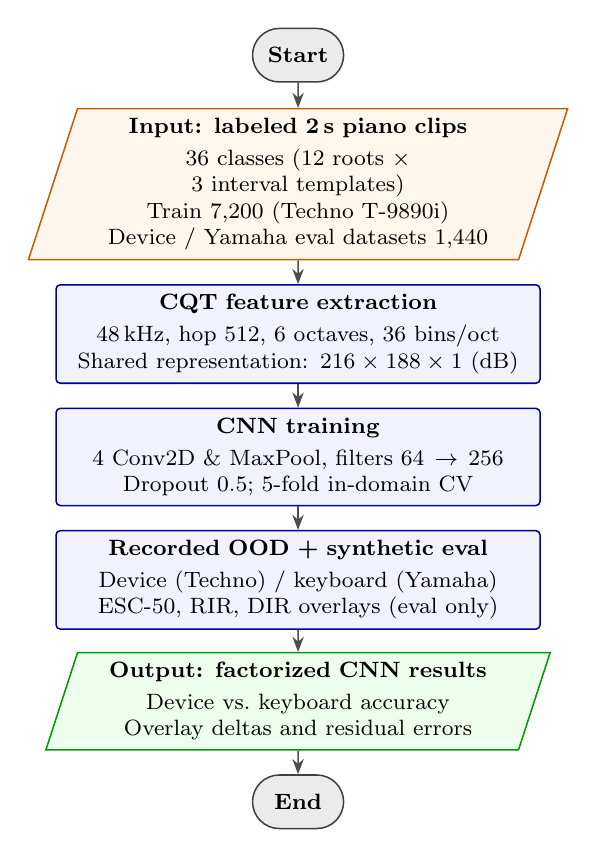
\begin{tikzpicture}[
    node distance=0.18cm and 0.12cm,
    >={Stealth},
    font=\footnotesize,
    base/.style={draw, align=center, minimum height=0.55cm, line width=0.55pt, inner sep=3.5pt},
    terminal/.style={base, shape=rounded rectangle, rounded rectangle arc length=180, draw=black!75, fill=black!8, minimum height=0.68cm, minimum width=2.0cm, inner xsep=12pt, inner ysep=3pt, font=\footnotesize\bfseries},
    process/.style={base, rectangle, rounded corners=1.5pt, draw=blue!60!black, fill=blue!5, text width=5.9cm},
    io/.style={base, trapezium, trapezium left angle=72, trapezium right angle=108, trapezium stretches body=true, draw=orange!75!black, fill=orange!7, text width=5.25cm, inner xsep=5pt},
    result/.style={base, trapezium, trapezium left angle=72, trapezium right angle=108, trapezium stretches body=true, draw=green!60!black, fill=green!7, text width=5.25cm, inner xsep=5pt},
    arrow/.style={->, line width=0.55pt, black!70}
  ]
    \node[terminal] (start) {Start};
    \node[io, below=0.32cm of start] (in1)
    {\textbf{Input: labeled 2\,s piano clips}\\[2pt]
     36 classes (12 roots $\times$ 3 interval templates)\\
     Train 7{,}200 (Techno T-9890i)\\
     Device / Yamaha eval datasets 1{,}440};
    \node[process, below=0.3cm of in1] (p2)
    {\textbf{CQT feature extraction}\\[2pt]
     48\,kHz, hop 512, 6 octaves, 36 bins/oct\\
     Shared representation: $216 \times 188 \times 1$ (dB)};
    \node[process, below=0.3cm of p2] (cnn1)
    {\textbf{CNN training}\\[2pt]
     4 Conv2D \& MaxPool, filters $64 \to 256$\\
     Dropout 0.5; 5-fold in-domain CV};
    \node[process, below=0.3cm of cnn1] (p5)
    {\textbf{Recorded OOD + synthetic eval}\\[2pt]
     Device (Techno) / keyboard (Yamaha)\\
     ESC-50, RIR, DIR overlays (eval only)};
    \node[result, below=0.28cm of p5] (out)
    {\textbf{Output: factorized CNN results}\\[2pt]
     Device vs.\ keyboard accuracy\\
     Overlay deltas and residual errors};
    \node[terminal, below=0.3cm of out] (endn) {End};
    \draw[arrow] (start) -- (in1);
    \draw[arrow] (in1) -- (p2);
    \draw[arrow] (p2) -- (cnn1);
    \draw[arrow] (cnn1) -- (p5);
    \draw[arrow] (p5) -- (out);
    \draw[arrow] (out) -- (endn);
  \end{tikzpicture}%
  }
  \caption{Experimental pipeline. The CNN is trained once on Techno CQT features. Overlays hit evaluation datasets only; weights stay frozen.}
  \label{fig:methodology}
\end{figure}

\subsection{Two evaluation scenarios}\label{subsec3_0}

Scenario~1 (in-domain) holds instrument, room, and device fixed and asks whether the CQT space separates the 36 classes at all. Five-fold cross-validation on the 7{,}200 Techno takes is that upper bound.

Scenario~2 changes one factor at a time and tests the same trained CNN with no fine-tuning. Three device-only datasets keep the Techno T-9890i and change only the microphone (ThinkPad internal mic, Vivo phone, Flow X13). Two keyboard-shift datasets then swap the instrument to a Yamaha PSR-S910 while reusing the ThinkPad and Flow microphones already measured on the Techno. That pairing is the point: \texttt{thinkpad} versus \texttt{thinkpad-2} differs by keyboard, not by mic; \texttt{flow} versus \texttt{flow-2} does the same. Table~\ref{tab:scenarios} lists every dataset. Synthetic overlays (Section~\ref{subsec3_7}) hit all five 1{,}440-sample datasets. The CNN is never retrained.

\begin{table*}[t]
\caption{Recorded evaluation datasets. The CNN is trained on \texttt{training} and evaluated on every dataset.}\label{tab:scenarios}
\begin{tabular*}{\textwidth}{@{\extracolsep{\fill}}lllll@{}}
\toprule
Dataset & $N$ & Primary shift & Instrument & Recording device \\
\midrule
\texttt{training} & 7{,}200 & None (in-domain) & Techno T-9890i & Xiaomi Redmi Pad 2 \\
\texttt{thinkpad} & 1{,}440 & Device & Techno T-9890i & ThinkPad mic \\
\texttt{vivo} & 1{,}440 & Device & Techno T-9890i & Vivo phone mic \\
\texttt{flow} & 1{,}440 & Device & Techno T-9890i & Flow X13 mic \\
\texttt{thinkpad-2} & 1{,}440 & Keyboard & Yamaha PSR-S910 & ThinkPad mic \\
\texttt{flow-2} & 1{,}440 & Keyboard & Yamaha PSR-S910 & Flow X13 mic \\
\bottomrule
\end{tabular*}
\end{table*}

\subsection{Dataset acquisition}\label{subsec3_1}

A web recorder sends simultaneous MIDI note-on events over USB and captures the microphone. That removes manual playing errors and keeps the instrument's physical resonance and synthesis. The same trigger list and voicing are used for every dataset, so class identity does not change with the acoustic condition.

The vocabulary is 36 classes. Each class is a three-note piano sound: one of 12 roots (C, C$\sharp$, \ldots, B) times one of three interval templates (maj $+4,+3$; min $+3,+4$; dim $+3,+3$ semitones). A semitone is one chromatic step and occupies three CQT bins. Figures write \emph{C maj}, \emph{E dim}; file names keep the fourth-octave suffix. All takes sit in that octave, inside C1--C7 ($\approx$33--2093\,Hz) \cite{Telila2023}\cite{Harte2010}. The dim template places its three notes closer together than maj or min \cite{Byambatsogt2020}. Both instruments use a grand-piano preset; they still differ in sample set, loudspeaker, and cabinet.

\begin{enumerate}[1.]
\item \textbf{Training (\texttt{training})}: 200 samples per class, 7{,}200 total. Xiaomi Redmi Pad 2 mic, Techno T-9890i Acoustic Grand Piano. Attack delays 0--150\,ms approximate keystroke asynchrony \cite{Bella2011}. OGG/OPUS, 48{,}000\,Hz, 32-bit, mono, no filters.
\item \textbf{Device-shift (\texttt{thinkpad}, \texttt{vivo}, \texttt{flow})}: 40 per class, 1{,}440 each, WAV. Techno T-9890i on ThinkPad, Vivo phone, and Flow X13 mics.
\item \textbf{Keyboard-shift (\texttt{thinkpad-2}, \texttt{flow-2})}: 40 per class, 1{,}440 each, WAV. Yamaha PSR-S910 on the ThinkPad and Flow mics already used on the Techno.
\end{enumerate}

No evaluation clip enters training, validation, early stopping, or hyperparameter choice.

\subsection{CQT feature extraction}\label{subsec3_2}

We compute CQT with \texttt{librosa.cqt()}. Each bin $f_k$ has constant quality
\begin{equation}
Q = \frac{f_k}{f_{k+1} - f_k} = \frac{1}{2^{1/B} - 1}
\label{eq:cqt}
\end{equation}
where $B$ is bins per octave \cite{Li2021}\cite{Lacoste2007}. Logarithmic spacing lines bins up with semitones, so a transposition is a vertical shift and a major third is the same bin distance on every root \cite{Harte2010}.

Table~\ref{tab:cqt-extraction-params} lists parameters. Thirty-six bins per octave (3 per semitone) resolve major ($+4,+3$), minor ($+3,+4$), and diminished ($+3,+3$) intervals \cite{Akram2025}\cite{OHanlon2021}. Each clip is truncated to a fixed 2.0\,s. Equation~\ref{eq:frames} gives 188 frames and a uniform shape $216 \times 188 \times 1$. Magnitudes go to dB with \texttt{librosa.amplitude\_to\_db(..., ref=np.max)}. The same parameters are used for training, every recorded dataset, and every overlay.

\begin{equation}
\text{frames} = \frac{\text{duration} \times \text{sample rate}}{\text{hop size}}
\label{eq:frames}
\end{equation}

\begin{table}[t]
\caption{CQT feature extraction parameters}\label{tab:cqt-extraction-params}
\begin{tabular}{@{}ll@{}}
\toprule
Parameter & Value \\
\midrule
Sample rate & 48{,}000\,Hz \\
Hop size & 512 samples \\
Octaves & 6 \\
Bins per octave & 36 \\
Total bins & 216 \\
Frequency range & C1 (32.70\,Hz) to C7 (2{,}093\,Hz) \\
Window & Hann \\
Frame length & 188 \\
Output shape & $216 \times 188 \times 1$ \\
\bottomrule
\end{tabular}
\end{table}

\subsection{CNN architecture and training}\label{subsec3_3}

The CNN follows Wolf-Monheim \cite{Wolf-Monheim2025}, originally designed for environmental sound classification on ESC-50. Its compact four-block convolutional structure without recurrent layers or attention is appropriate for fixed-window classification from static spectrograms.

Table~\ref{tab:cnn-architecture} lists layers. Input batch normalization matches CQT magnitude statistics across samples and recording conditions, which matters when later datasets use different microphones and a different piano. The four Conv2D--MaxPooling2D blocks build a progressive hierarchy: the first block (64 filters) captures low-level spectral texture; the second (128 filters) encodes mid-level harmonic interval patterns; the third and fourth (256 filters each) represent chord-quality abstractions. The $3\times3$ receptive field matches the 1--2 bin frequency shifts that distinguish chord types, while MaxPooling provides spatial subsampling and limited translation invariance \cite{Purwono2022}. Dropout (rate 0.5) limits co-adaptation to the Techno piano voice.

\begin{table}[t]
\caption{CNN architecture specification}\label{tab:cnn-architecture}
\begin{tabularx}{\columnwidth}{@{}lXl@{}}
\toprule
Layer & Output shape & Notes \\
\midrule
BatchNorm & $216{\times}188{\times}1$ & Input normalization \\
Conv2D & $216{\times}188{\times}64$ & $3{\times}3$, ReLU, same \\
MaxPool & $108{\times}94{\times}64$ & $2{\times}2$, stride 2 \\
Conv2D & $108{\times}94{\times}128$ & $3{\times}3$, ReLU, same \\
MaxPool & $54{\times}47{\times}128$ & $2{\times}2$, stride 2 \\
Conv2D & $54{\times}47{\times}256$ & $3{\times}3$, ReLU, same \\
MaxPool & $27{\times}23{\times}256$ & $2{\times}2$, stride 2 \\
Conv2D & $27{\times}23{\times}256$ & $3{\times}3$, ReLU, same \\
MaxPool & $13{\times}11{\times}256$ & $2{\times}2$, stride 2 \\
Flatten & 36{,}608 & \\
Dense & 256 & ReLU \\
Dropout & 256 & rate 0.5 \\
Dense & 36 & Softmax \\
\bottomrule
\end{tabularx}
\end{table}

Training follows Table~\ref{tab:cnn-training-config}. Stratified 80/10/10 sampling with seed 42 keeps class balance. \texttt{ReduceLROnPlateau} multiplies the learning rate by 0.1 after 2 stagnant val-loss epochs; \texttt{EarlyStopping} stops after 6; max 50 epochs \cite{Wolf-Monheim2025}. The 10\% test split is held out of training and validation. The same trained weights are used for every later test.

\begin{table}[t]
\caption{CNN training configuration}\label{tab:cnn-training-config}
\begin{tabular}{@{}ll@{}}
\toprule
Parameter & Value \\
\midrule
Random seed & 42 \\
Train / Val / Test split & 80\% / 10\% / 10\% \\
Batch size & 32 \\
Initial learning rate & 0.001 \\
Optimizer & Adam \\
Weight initialization & Glorot uniform \\
Loss & Categorical cross-entropy \\
Max epochs & 50 \\
EarlyStopping patience & 6 epochs \\
ReduceLROnPlateau & factor 0.1, patience 2 \\
\bottomrule
\end{tabular}
\end{table}

\subsection{5-fold cross-validation}\label{subsec3_5}

Five folds on all 7{,}200 training samples, 80/20 per fold, measure in-domain score independent of one train/test split. Each fold retrains the CNN from a fresh random initialization and a fixed per-fold seed. Fold test partitions never enter training or early stopping for that fold.

\subsection{Synthetic degradations (evaluation only)}\label{subsec3_7}

Three overlays hit already out-of-domain datasets without retraining. Overlay probability is 1 (every evaluation sample is degraded), the draw is random per sample with a fixed seed, and wet waveforms are not written back into the training tree. The same five datasets are used for all three overlays, so deltas are comparable.

\textbf{Additive noise.} ESC-50 interior/domestic clips \cite{Piczak2015} are converted to CQT with the same hop and binning as the chord features, yielding a 400-clip bank over 10 classes. Mixing is performed in the CQT power domain at a uniform SNR drawn from $[10, 25]$\,dB (realized mean 17.5\,dB) with a random time roll. This is a controlled interior overlay, not a claim that ESC-50 matches any one room.

\textbf{Room impulse responses.} Indoor IRs from the McDermott IR Survey \cite{Traer2016} are resampled to 48\,kHz and trimmed of leading silence. Bathrooms, showers, and outdoor/transit rooms are excluded, leaving 174 indoor IRs. Each evaluation waveform is convolved with a randomly drawn IR, cropped, peak-normalized, and converted to CQT.

\textbf{Device impulse responses.} Six measured microphone IRs (AKG D12, Crystal, Lomo 52A-5M, Melodium RM6, Oktava MD57, STC 4035) are preprocessed identically and convolved one-per-sample onto the same five datasets. They probe extra mic colouring on top of the already recorded consumer microphones.

These overlays test a clean-trained CQT--CNN. They are not a training recipe, and they are applied independently: a noise trial does not also convolve an IR, so the three columns of Table~\ref{tab:aug} remain single-factor.

\subsection{Evaluation metrics}\label{subsec3_6}

Accuracy, precision, recall, and F1 come from the confusion matrix. For a one-versus-rest partition of a single class the counts are True Positives (TP), True Negatives (TN), False Positives (FP), and False Negatives (FN):
\begin{equation}
\mathrm{P}=\frac{\mathrm{TP}}{\mathrm{TP}+\mathrm{FP}},\quad
\mathrm{R}=\frac{\mathrm{TP}}{\mathrm{TP}+\mathrm{FN}},\quad
\mathrm{F1}=\frac{2\mathrm{PR}}{\mathrm{P}+\mathrm{R}}.
\label{eq:prf}
\end{equation}
Accuracy is the fraction of clips with the correct label. Macro P, R, and F1 are unweighted means over the 36 classes. On the Yamaha datasets, macro F1 falls below accuracy because a few destination classes absorb false positives. Per-class recall and off-diagonal counts show which qualities collapse after a microphone or keyboard change.

\section{Results}\label{sec4}

\subsection{CQT feature extraction}\label{subsec4_1}

\begin{figure}[t]
\centering
\includegraphics[width=\columnwidth]{fig-cqt-train.png}
\caption{Training CQT of C maj ($+4,+3$) and C min ($+3,+4$): same root, one-semitone gap in the middle note. Frequency in Hz.}
\label{fig:cqt-spectrograms}
\end{figure}

Every clip becomes a $216 \times 188$ CQT dB matrix. Fig.~\ref{fig:cqt-spectrograms} shows C maj and C min from the training set: same root, one semitone (three CQT bins) in the middle note.

\subsection{In-domain cross-validation performance}\label{subsec4_2}

Under Scenario~1 the CNN scores 1.00 accuracy, precision, recall, and F1 on every fold of the 7{,}200 Techno takes. Resubstitution on the full training dataset is 0.9999: one $C$ diminished clip is predicted $C$ minor. With instrument, room, and device fixed, the CQT space separates all 36 classes. Later drops are therefore a domain-shift cost, not a capacity or representation failure of this architecture on this vocabulary.

\subsection{Factorized recorded shifts}\label{subsec4_3}

Table~\ref{tab:cross-domain} and Fig.~\ref{fig:cross-domain} score the frozen CNN on every recorded dataset. Device-only datasets keep the Techno and change the microphone: \texttt{thinkpad} 0.994 accuracy / 0.994 F1, \texttt{vivo} 0.946 / 0.937, \texttt{flow} 0.944 / 0.935. Keyboard-shift datasets swap in the Yamaha PSR-S910: \texttt{thinkpad-2} 0.885 / 0.856, \texttt{flow-2} 0.874 / 0.840. Switching the instrument accounts for most of the recorded drop. The ThinkPad mic that was nearly perfect on the Techno (0.994) falls to 0.885 on the Yamaha, a 10.9-point gap on a matched mic. The Flow pairing repeats the pattern: 0.944 $\to$ 0.874 (7.0 points). On the Yamaha datasets, precision (0.849 and 0.848) sits below recall, so F1 undershoots accuracy: a few destination classes absorb the collapsed sources.

\begin{table}[t]
\caption{Fixed CNN on recorded datasets. Precision, recall, and F1 are macro averages.}\label{tab:cross-domain}
\setlength{\tabcolsep}{3.5pt}
\begin{tabular}{@{}llrrrr@{}}
\toprule
Dataset & Shift & Acc. & P & R & F1 \\
\midrule
\texttt{training} & In-domain & 0.9999 & 1.000 & 1.000 & 1.000 \\
\texttt{thinkpad} & Device & 0.994 & 0.995 & 0.994 & 0.994 \\
\texttt{vivo} & Device & 0.946 & 0.950 & 0.946 & 0.937 \\
\texttt{flow} & Device & 0.944 & 0.964 & 0.944 & 0.935 \\
\texttt{thinkpad-2} & Keyboard & 0.885 & 0.849 & 0.885 & 0.856 \\
\texttt{flow-2} & Keyboard & 0.874 & 0.848 & 0.874 & 0.840 \\
\bottomrule
\end{tabular}
\end{table}

\begin{figure}[t]
\centering
\includegraphics[width=\columnwidth,height=0.26\textheight,keepaspectratio]{fig-cross-domain.pdf}
\caption{Fixed CNN accuracy on the training dataset and five held-out datasets.}
\label{fig:cross-domain}
\end{figure}

Mean per-class recall by quality (12 classes each) shows the same concentration. Major and minor stay high after a microphone change. Diminished already slips on \texttt{vivo} (0.915) and \texttt{flow} (0.890), then falls to 0.765 / 0.790 on the Yamaha. Major recall on \texttt{thinkpad-2} remains 0.975. The keyboard factor is not a uniform 11-point tax on every class.

Fig.~\ref{fig:perclass} shows the nine classes that drop on each matched-mic pair. On the ThinkPad, Techno stays high ($E$ dim 0.925, $C$ maj 0.875). The same mic on the Yamaha zeros $D$ min, $E$ dim, and $G\sharp$ dim, and cuts $A\sharp$ dim to 0.525 and $C$ dim to 0.700. The Flow pairing agrees on those three zero-recall Yamaha classes and adds a $B$ maj miss (0.125).

\begin{figure*}[t]
\centering
\includegraphics[width=0.92\textwidth,height=0.28\textheight,keepaspectratio]{fig-perclass-paired.pdf}
\caption{Per-class recall on matched microphones for the classes that drop.
\textbf{(A)}~ThinkPad. \textbf{(B)}~Flow X13.
Microphone fixed, instrument swapped. The other 27 classes are 1.00 on both instruments.}
\label{fig:perclass}
\end{figure*}

Table~\ref{tab:pairs} lists the largest off-diagonal cells. Device-shift errors on \texttt{vivo} and \texttt{flow} run through $E$ minor. Keyboard-shift errors change destination: $D$ minor $\to$ $B$ diminished, $E$ diminished $\to$ $D$/$D\sharp$ major, $G\sharp$ diminished $\to$ $B$ minor/$G$ major, and $B$ major $\to$ $A\sharp$ minor on \texttt{flow-2}.

\begin{table*}[t]
\caption{Largest off-diagonal counts (40 takes per class). Notes are the three pitch classes of each triad; shared notes are in both.}\label{tab:pairs}
\setlength{\tabcolsep}{3.5pt}
\begin{tabular*}{\textwidth}{@{\extracolsep{\fill}}lllllllr@{}}
\toprule
Dataset & Shift & True & True notes & Pred. & Pred.\ notes & Shared & $n$ \\
\midrule
\texttt{vivo} & Device & $E$ dim & $E,G,A\sharp$ & $E$ min & $E,G,B$ & $E,G$ & 40 \\
\texttt{vivo} & Device & $C$ maj & $C,E,G$ & $E$ min & $E,G,B$ & $E,G$ & 29 \\
\texttt{flow} & Device & $E$ dim & $E,G,A\sharp$ & $E$ min & $E,G,B$ & $E,G$ & 36 \\
\texttt{flow} & Device & $B$ maj & $B,D\sharp,F\sharp$ & $G$ min & $G,A\sharp,D$ & --- & 19 \\
\texttt{flow} & Device & $C\sharp$ dim & $C\sharp,E,G$ & $C\sharp$ min & $C\sharp,E,G\sharp$ & $C\sharp,E$ & 16 \\
\texttt{thinkpad-2} & Keyboard & $D$ min & $D,F,A$ & $B$ dim & $B,D,F$ & $D,F$ & 40 \\
\texttt{thinkpad-2} & Keyboard & $G\sharp$ dim & $G\sharp,B,D$ & $B$ min & $B,D,F\sharp$ & $B,D$ & 25 \\
\texttt{thinkpad-2} & Keyboard & $E$ dim & $E,G,A\sharp$ & $D$ maj & $D,F\sharp,A$ & --- & 23 \\
\texttt{flow-2} & Keyboard & $D$ min & $D,F,A$ & $B$ dim & $B,D,F$ & $D,F$ & 39 \\
\texttt{flow-2} & Keyboard & $E$ dim & $E,G,A\sharp$ & $D$ maj & $D,F\sharp,A$ & --- & 37 \\
\texttt{flow-2} & Keyboard & $B$ maj & $B,D\sharp,F\sharp$ & $A\sharp$ min & $A\sharp,C\sharp,F$ & --- & 35 \\
\texttt{flow-2} & Keyboard & $G\sharp$ dim & $G\sharp,B,D$ & $G$ maj & $G,B,D$ & $B,D$ & 25 \\
\bottomrule
\end{tabular*}
\end{table*}

\subsection{Synthetic degradations}\label{subsec4_5}

Table~\ref{tab:aug} and Fig.~\ref{fig:aug} compare clean accuracy with ESC-50 noise, indoor RIR, and microphone DIR. Weights stay frozen. Additive noise always hurts (0.8--4.9 accuracy points; 0.9--4.3 F1). The largest drop is on Yamaha dataset \texttt{thinkpad-2} (0.885 $\to$ 0.837; F1 0.856 $\to$ 0.813). Room convolution is mixed: \texttt{vivo} $-4.9$, \texttt{thinkpad} $-2.7$, \texttt{flow} $+0.6$. Device IRs are near zero on four datasets and lift \texttt{flow} from 0.944 to 0.978.

\begin{table*}[t]
\caption{CNN accuracy under eval-only overlays. Parentheses: degraded minus clean, percentage points.}\label{tab:aug}
\begin{tabular*}{\textwidth}{@{\extracolsep{\fill}}lrrrr@{}}
\toprule
Dataset & Clean & Noise & RIR & DIR \\
\midrule
\texttt{thinkpad} & 0.994 & 0.960 ($-3.5$) & 0.967 ($-2.7$) & 0.989 ($-0.6$) \\
\texttt{vivo} & 0.946 & 0.910 ($-3.5$) & 0.897 ($-4.9$) & 0.948 ($+0.2$) \\
\texttt{flow} & 0.944 & 0.935 ($-0.8$) & 0.950 ($+0.6$) & 0.978 ($+3.5$) \\
\texttt{thinkpad-2} & 0.885 & 0.837 ($-4.9$) & 0.867 ($-1.8$) & 0.874 ($-1.2$) \\
\texttt{flow-2} & 0.874 & 0.842 ($-3.3$) & 0.874 ($-0.1$) & 0.875 ($+0.1$) \\
\bottomrule
\end{tabular*}
\end{table*}

\begin{figure*}[t]
\centering
\includegraphics[width=0.88\textwidth,height=0.18\textheight,keepaspectratio]{fig-aug-compare.pdf}
\caption{Eval-only overlays on the five held-out datasets: additive interior noise, indoor room IR, extra microphone IR.}
\label{fig:aug}
\end{figure*}

\section{Discussion}\label{sec5}

\subsection{Device shift versus keyboard shift}\label{subsec5_0}

Hold the Techno T-9890i and change only the consumer microphone: accuracy stays in 0.944--0.994. The ThinkPad internal mic is almost an in-domain clone of the Redmi Pad 2 training mic. The Vivo phone and Flow X13 cost about five points each, and those points sit on a handful of classes (Section~\ref{subsec5_1}).

Switch the instrument to the Yamaha PSR-S910 on a microphone already scored on the Techno, and accuracy falls 10.9 points (\texttt{thinkpad} $\to$ \texttt{thinkpad-2}) and 7.0 points (\texttt{flow} $\to$ \texttt{flow-2}). The two Yamaha datasets also agree (0.885 vs.\ 0.874), so the drop tracks the keyboard. Timbre and voice synthesis move the harmonic template more than the colouring of these three consumer microphones. A new phone or laptop on the Techno transfers. The Yamaha grand-piano voice does not, at least not to the 0.94 floor the device datasets reach. Shipping the same model to a second microphone on the same keyboard is cheap. Shipping it to a second keyboard, even with a grand-piano preset and the same MIDI voicing, needs more instruments in the training mix or an adaptation step.

\subsection{CNN error structure under domain shift}\label{subsec5_1}

Errors cluster on close triads; they do not spread across the 36-way matrix. On device-shift \texttt{vivo}, all 40 $E$ diminished takes are labelled $E$ minor. Dataset \texttt{flow} sends 36 of 40 the same way and adds 16 $C\sharp$ diminished $\to$ $C\sharp$ minor. Those pairs share the root and fifth and differ by one semitone in the third (three CQT bins). The Vivo dataset also sends 29 of 40 $C$ major takes into $E$ minor, the relative minor, sharing $E$ and $G$. $E$ minor precision falls to 0.367 while its recall stays 1.00.

On both Yamaha datasets, $D$ minor, $E$ diminished, and $G\sharp$ diminished have zero recall. $D$ minor ($D$, $F$, $A$) is labelled $B$ diminished ($B$, $D$, $F$) on 40 ThinkPad takes and 39 Flow takes; those triads share $D$ and $F$. $B$ diminished precision falls to 0.40 / 0.41 because it also collects 19 and 18 $A\sharp$ diminished takes. $G\sharp$ diminished splits between $B$ minor and $G$ major, each sharing two pitch classes. $E$ diminished goes to $D$ major and $D\sharp$ major rather than $E$ minor. On \texttt{flow-2}, 35 of 40 $B$ major takes land on $A\sharp$ minor, a one-semitone slide of the whole chord. $E$ diminished is the weakest class on every OOD dataset (0.925 on \texttt{thinkpad}, 0 on \texttt{vivo} and both Yamaha datasets, 0.075 on \texttt{flow}). A later training mix should oversample that quality rather than treating all 36 labels as equally hard.

\subsection{Synthetic overlays versus recorded keyboard shift}\label{subsec5_2}

ESC-50 interior mixing never drops a Techno device dataset below 0.910 accuracy. The same overlay on Yamaha \texttt{thinkpad-2} reaches 0.837, the lowest cell in Table~\ref{tab:aug}. Keyboard change and additive noise stack: the 4.9-point noise tax sits on top of the 10.9-point Yamaha tax already paid on that mic.

Edwards et al.\ \cite{Edwards2024} applied test-time noise and reverb to a clean-trained transcription model and saw drops of several to about 19 note-onset F1 points on MAPS, then recovered the OOD set with train-time mixing. Our eval-only noise tax is smaller: isolated 2\,s triads at 10--25\,dB SNR leave the harmonic stack visible, whereas their onset metric is sensitive to masking. The ordering still matches. Additive noise is the most consistent eval-only harm; a random indoor IR can help or hurt; an extra microphone IR is the weakest change, except the $+3.5$ lift on \texttt{flow}. That gain is a chance move of the Flow spectrum toward the training envelope. It is not a pre-process to ship, and it does not close the Yamaha gap (\texttt{flow-2} DIR is $+0.1$). None of the overlays trained the model. Closing the remaining Yamaha and $E$ diminished errors is a training-set problem: more piano voices, or an Edwards-style mix applied while the CNN still updates.

\subsection{Limitations}\label{subsec5_3}

Both instruments are digital pianos on a grand-piano preset; an acoustic grand would be a larger keyboard factor. All voicings are isolated fourth-octave triads. Training uses one tablet microphone. ESC-50, the McDermott indoor IRs, and the six measured DIRs are controlled overlays, not a match to any one target room. The study reports one compact CNN.

\section{Conclusion}\label{sec6}

A compact CQT--CNN reaches 1.00 in-domain on 36 Techno T-9890i piano chords. A new consumer microphone on the same Techno leaves 0.944--0.994 accuracy. Switching to the Yamaha PSR-S910, on microphones already scored on the Techno, drops accuracy to 0.874--0.885 and macro F1 to 0.840--0.856. The cost is concentrated on diminished classes: $D$ minor, $E$ diminished, and $G\sharp$ diminished have zero recall on both Yamaha datasets. Eval-only ESC-50 noise subtracts 0.8--4.9 accuracy points and stacks with the keyboard gap. Indoor RIR and microphone DIR move the score by less, and sometimes raise it. Residual errors stay on shared-tone or one-semitone neighbours, above all $E$ diminished.

We withheld train-time mixing so these numbers remain a factorized baseline: device versus keyboard, then matched overlays. Edwards et al.\ \cite{Edwards2024} recover OOD piano transcription with noise and reverb mixing at train time. That is the next chord step, together with more piano voices and a vocabulary beyond fourth-octave triads. Score those steps against this baseline, not against in-domain 1.00.

\backmatter

\bmhead{Author contributions}
All authors contributed to study conceptualization and design. Material preparation, data acquisition, experimentation, analysis, and drafting were performed by CGS. All authors reviewed and approved the final version.

\bmhead{Funding}
No funding was received for this work.

\bmhead{Data availability}
The piano chord dataset is publicly available at \url{https://zenodo.org/records/21077144}.

\bmhead{Code availability}
The dataset generation and recording tool is available at \url{https://github.com/sglkc/chords-dataset-generator/}. Experiment notebooks are available in the project repository.

\section*{Declarations}

\bmhead{Conflict of interest}
The authors declare no competing interests.

\bmhead{Ethics approval}
Not applicable.

\bmhead{Consent for publication}
All authors approved the final manuscript.

\bibliography{mendeley}

\end{document}
